\documentclass{beamer}
  
\usepackage[utf8]{inputenc}
\usepackage[portuges]{babel}
\usepackage{lmodern, comment}
\usepackage{graphicx}
\usepackage{xcolor}
\usepackage{pifont}
 \usepackage{listings}
%%%\usepackage[]{minted}  
 
\usetheme{default}
\usefonttheme{default}
\usecolortheme{default}
\useinnertheme{default}
\useoutertheme{default}

\usetheme{Boadilla}

\begin{comment} 
\usetheme[width=15mm]{Berkeley}
%%largura da pagina ao lado
\makeatletter\beamer@headheight=0.06\textheight

%\usecolortheme{sidebartab}
%%\useoutertheme[width=58pt,height=25pt,right,hideothersubsections]{sidebar}
\useinnertheme{rounded}
\setbeamercolor{title}{bg=red!25!blue,fg=white}
\setbeamercolor{fo} {bg=red!25!blue,fg=white}
\setbeamercolor{sidebar}{bg=red!25!blue,fg=white}
\setbeamercolor{author in sidebar}{fg=black!20!white}
\setbeamercolor{title in sidebar}{fg=white}
\setbeamercolor{normal text}{bg=white}
\setbeamercolor{frametitle}{bg=blue!40!white , fg=yellow}
\setbeamercolor{section in sidebar}{bg=black,fg=yellow}
\setbeamercolor{subsection in sidebar}{bg=black,fg=white}
\setbeamercolor{block title}{bg=red!25!blue,fg=white}
\setbeamercolor{block body}{bg=blue!20!white,fg=black}
\setbeamerfont{subsection in sidebar}{size=\tiny}
\setbeamerfont{title in sidebar}{size=\scriptsize}
\setbeamerfont{title in frametitle}{size=\normalsize}%% nao funciona
\setbeamerfont{author in sidebar}{size=\tiny}
\setbeamercovered{transparent}
\setbeamertemplate{blocks}[rounded][shadow=true]
\end{comment}


%\setbeamertemplate{footline}
%{
%\begin{beamercolorbox}[wd=1\paperwidth,ht=0.05\textheight,dp=1ex,right]{fo}
%\insertframenumber{} / \inserttotalframenumber\hspace*{2ex}
%  \end{beamercolorbox}
%}

%%% FIGURAS
\graphicspath{{../figuras/}{../../figuras/}}
%%%%\graphicspath{ {/home/user} } {/home/ccs/Dropbox/main_ccs/livro_pr_modelos/}

\title[Modelos em PR -- Estudo de Caso] % (optional, use only with long paper titlebg=blue!20!white,s)
{Modelos em PR -- Estudo de Caso: \\ Uma Apresentação}

%\subtitle
%{About some things}

\author[Claudio Cesar de Sá] % (optional, use only with lots of authors)
{Claudio Cesar de Sá\inst{1}}
% - Give the names in the same order as the appear in the paper.
% - Use the \inst{?} command only if the authors have different
%   affiliation.

\institute[] % (optional, but mostly needed)
{
  \inst{1}%
  Departamento de Ciência da Computação -- DCC\\
  Centro de Ciências Tecnológicas -- CCT\\
 Universidade do Estado de Santa Catarina -- UDESC
}
% - Use the \inst command only if there are several affiliations.
% - Keep it simple, no one is interested in your street address.

\date[01 out 2015] % (optional, should be abbreviation of conference name)
{Projeto de um Livro -- Modelos em PR\\
CCT--UDESC\\ Outubro de 2015 -- SC}
% - Either use conference name or its abbreviation.
% - Not really informative to the audience, more for people (including
%   yourself) who are reading the slides online

\subject{Theoretical Computer Science}
% This is only inserted into the PDF information catalog. Can be left
% out. 


% If you have a file called "university-logo-filename.xxx", where xxx
% is a graphic format that can be processed by latex or pdflatex,
% resp., then you can add a logo as follows:

%\pgfdeclareimage[height=0.5cm]{cor_vertical_rgb.jpg}{cor_horizontal_rgb.jpg}
 %\logo{\pgfuseimage{cor_horizontal_rgb.jpg}}
%\pgfdeclareimage[height=0.5cm]{institution-logo}{cor_horizontal_rgb.jpg}
%\logo{\pgfuseimage{cor_horizontal_rgb.jpg}}

 

% If you wish to uncover everything in a step-wise fashion, uncomment
% the following command: 

%\beamerdefaultoverlayspecification{<+->}


\begin{document}

\begin{frame}
  \titlepage
\end{frame}



% Structuring a talk is a difficult task and the following structure
% may not be suitable. Here are some rules that apply for this
% solution: 

% - Exactly two or three sections (other than the summary).
% - At *most* three subsections per section.
% - Talk about 30s to 2min per frame. So there should be between about
%   15 and 30 frames, all told.

% - A conference audience is likely to know very little of what you
%   are going to talk about. So *simplify*!
% - In a 20min talk, getting the main ideas across is hard
%   enough. Leave out details, even if it means being less precise than
%   you think necessary.
% - If you omit details that are vital to the proof/implementation,
%   just say so once. Everybody will be happy with that.

%%%%%%%%%%%%%%%%%%%%%%%%%%%%%%%%%%%%%%%%%%%%%%%%%%%%%%%



%%%%%%%%%%%%%%%%%%%%%%%%%%%%%%%%%%%%%%%%%%%%%%%%%%%%%
\section{Um Exemplo de Problema Dificil: Cabo de Guerra}


\begin{frame}
\frametitle{Um Problema Difícil (NP): Cabo de Guerra}

\begin{figure}[ht!]
 \centering
 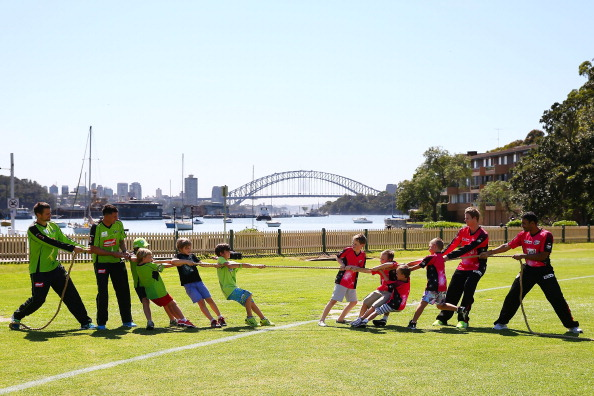
\includegraphics[width=0.8\textwidth , height=0.6\textheight]{cabo-de-guerra.jpg}
% \caption{} 
%\label{}
\end{figure}


\end{frame}

%%%%%%%%%%%%%%%%%%%%%%%%%%%%%%%%%%%%%%%%%%%%%%%%%%%%%%%%%%%%%%%%

\begin{frame}
\frametitle{Critério de escolha do times: por peso}

\begin{figure}[ht!]
 \centering
 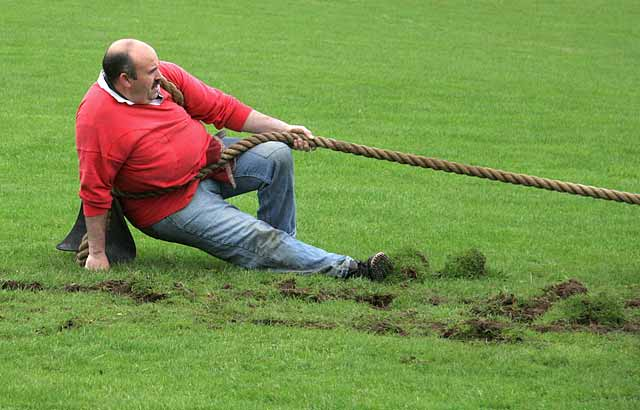
\includegraphics[width=0.7\textwidth , height=0.7\textheight]{separar_por_peso02.jpg}
\caption{\textit{O mais pesado tem mais força!}} 
%\label{}
\end{figure}

\end{frame}

%%%%%%%%%%%%%%%%%%%%%%%%%%%%%%%%%%%%%%%%%%%%%%%%%%%%%%%%%%%%%

\begin{frame}
\frametitle{Especificando o problema do Cabo de Guerra}

\begin{block}{Que seja feita a divisão:}


 
\begin{center}
\begin{tabular}{|c|c|c|c|c|}
\hline
$Joao_1$ & $Pedro_2$ & $Manoel_3$ & .... & $Zeca_n$ \\ \hline
45 & 39 & 79 & .... & 42  \\ \hline
\end{tabular}
\end{center}

\begin{itemize}
\item Divisão  por peso
\item Respeitar  critérios como: $|N_A - N_B| \le 1$
\item Todos devem brincar

\item \textsf{Bem, esta simples {\bf \underline{restrição}} ({\bf $|N_A - N_B| \le 1$}), de nosso cotidiano tornou um simples problema em mais uma questão combinatória.
 Um arranjo da ordem de  $\frac{n!}{(n/2)!}$.
 Casualmente, nada trivial  para grandes valores! }
 \end{itemize}
 
\end{block}
\end{frame}
%%%%%%%%%%%%%%%%%%%%%%%%%%%%%%%%%%%%%%%%%%%%%%%%%


\subsection{Modelagem}

\begin{frame}
\frametitle{Estratégia de Modelagem}
\begin{block}{}
  \begin{itemize}
  \item Variável de Decisão: análogo a árvore do SAT  
 
\begin{center}
\begin{tabular}{|l|c|c|c|c|c|}
\hline
Nomes ($n_i$): & $n_1$ & $n_2$ & $n_3$ & .... & $n_n$ \\ \hline
Peso ($p_i$): & 45 & 39 & 79 & .... & 42  \\ \hline
Binária ($x_i$): & 0/1 & 0/1 & 0/1 & .... & 0/1  \\ \hline
\end{tabular}
\end{center}
  
\item Assim $N_A \approx N/2$, $N_B \approx N/2$  e  $|N_A - N_B| \le 1$   

\item $x_i = 0$: $n_i$ fica para o time $A$
\item $x_i = 1$: $n_i$ fica para o time $B$
\item Logo a soma:
$$\sum_{i=1}^n x_i p_i$$ é o peso total do time $B$ ($P_B$)
  
  \end{itemize}
\end{block}
\end{frame}

%%%%%%%%%%%%%%%%%%%%%%%%%%%%%%%%%%%%%%%%%%%%%%%%%
\subsection{Modelagem}

\begin{frame}
\frametitle{Modelagem das Restrições}
\begin{block}{}
  \begin{itemize}
  \item Falta encontrar peso total do time $A$ ($P_A$), dado por: 

  \item $P_A = P_{total} - P_B$
  
  \item  ou $$P_A = \sum_{i=1}^n p_i - \sum_{i=1}^n x_i p_i$$   

  \item Finalmente, aplicar uma minimização  na diferença: $|P_A - P_B|$
  
%%  \item A seguir, tudo isto em código:
  
  \end{itemize}
\end{block}
\end{frame}

%%%%%%%%%%%%%%%%%%%%%%%%%%%%%%%%%%%%%%%%%%%%%%%%%
\subsection{Uma Estratégia de Implementação}

\begin{frame}[fragile]
\frametitle{Uma Estratégia de Implementação}
%\begin{block}{Código do Cabo de Guerra (um NP mesmo!)}

\begin{figure}[ht!]
 \centering
 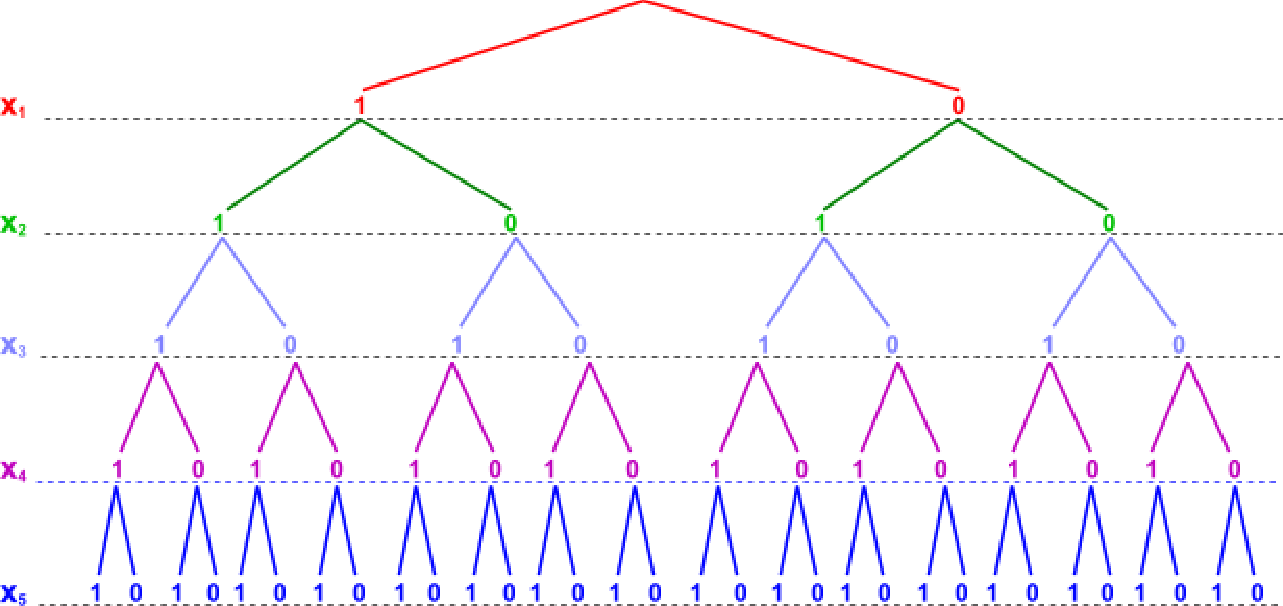
\includegraphics[width=0.9\textwidth , height=0.7\textheight]{../figuras/binary_tree04.pdf}
\caption{Se $x_i=0$, então $n_i$ segue para o time $A$, caso  $x_i=1$, então  $n_i$ vai para o time $B$} 
%\label{}
\end{figure}

\vspace{-1cm}
\begin{center}
\textcolor{red}{Qual a técnica  usada?}
\end{center}
%\end{block}

\end{frame}

%%%%%%%%%%%%%%%%%%%%%%%%%%%%%%%%%%%%%%%%%%%%%%%%%
\subsection{Implemetação em Minizinc}

\begin{frame}[fragile]
\frametitle{Implementação em Minizinc}

%\inputminted[linenos, numbersep=5pt, tabsize=4, frame=lines, label=cabo_de_guerra.scala]
{\small
%\inputminted{scala}{cabo_de_guerra01.scala}
}
\end{frame}

%%%%%%%%%%%%%%%%%%%%%%%%%%%%%%%%%%%%%%%%%%%%%%%%%

\begin{frame}[fragile]
%\frametitle{Implementação em Minizinc}

%\inputminted[linenos, numbersep=5pt, tabsize=4, frame=lines, label=cabo_de_guerra.scala]
{\small
%\inputminted{scala}{cabo_de_guerra02.scala}
}
\end{frame}

%%%%%%%%%%%%%%%%%%%%%%%%%%%%%%%%%%%%%%%%%%%%%%%%%

\subsection{Resultados e Análise}
\begin{frame}
\frametitle{Resultados e Análise}
\begin{block}{Números aleatórios de 1 a 150}

Usando um \textit{solver} médio do Minizinc (\textit{G12 lazyfd}) padrão:

\begin{center}
  \begin{tabular}{ l | c |c | r }
    \hline  \hline 
    $n$ & tempo & $P_A$ & $P_B$\\ \hline     \hline 
     5 & 40msec & 276 & 278 \\ \hline
    10 & 46msec & 518 & 519 \\ \hline
    25 & 98msec & 1198 & 1197 \\ \hline
    50 & 411msec & 2290 & 2291 \\ \hline
    75 & \textbf{\textcolor{red}{2s 485msec}} & 3133 & 3133 \\ \hline
    100 & 470msec & 4142 & 4142 \\ \hline 
    125 & \textbf{\textcolor{red}{7s 2msec}} & 4992 & 4992 \\ \hline 
    150 & 605msec & 5823 & 5823 \\ \hline 
    175 & 642msec &   6777 &  6778 \\ \hline 
    200 & $>$ 10min & -- & -- \\ \hline \hline
  \end{tabular}
\end{center}

Referência: cpu 4-core, 4 G ram, SO: Linux-Debian


\end{block}
\end{frame}

%%%%%%%%%%%%%%%%%%%%%%%%%%%%%%%%%%%%%%%%%%%%%%%%%%%%%%%



%%%%%%%%%%%%%%%%%%%%%%%%%%%%%%%%%%%%%%%%%%%%%%%%%%%%
\subsection{Resumindo ... }

\begin{frame}
\frametitle{Reflexões}
\begin{block}{}   %%%%Implemetação em Minizinc
\begin{flushleft}

\vspace{1cm}
\ding{224} \textsf{Enfim, este problema é uma variação de clássicos
NPs, mais especificamente o \textit{sub-set-sum}}

\vspace{1cm}
\ding{224} \textsf{Leia-se: Problema da Mochila}


\vspace{1cm}
\ding{224} \textsf{Implemente este problema usando Programação Dinâmica (PD)}

      \end{flushleft}

    \end{block}
  \end{frame}

%%%%%%%%%%%%%%%%%%%%%%%%%%%%%%%%%%%%%%%%%%%%%%%%%%%%%%%



%%%%%%%%%%%%%%%%%%%%%%%%%%%%%%%%%%%%%%%%%%%%%%%%%%%%%%%



\end{document}
